\documentclass[10pt]{beamer}
\useoutertheme{infolines}
\useinnertheme{rectangles}
\usecolortheme{whale}
\usecolortheme{orchid}
\setbeamersize{text margin left=1cm,text margin right=1cm}
\setbeamertemplate{footline}{}
% \beamertemplatenavigationsymbolsempty

\usepackage[czech]{babel}

\AtBeginDocument{\renewcommand\vec{\mathbf}}
\usepackage{physics}
\renewcommand\dd[1]{\,\mathsf{d}#1}
\renewcommand\dv[2]{\frac{\text{d}#1}{\text{d}#2}}
\usepackage[version=4]{mhchem}
\mhchemoptions{textfontcommand=\sffamily}
\mhchemoptions{mathfontcommand=\mathsf}
\usepackage{siunitx}
\sisetup{
	locale               = DE,
	inter-unit-product   = \ensuremath{{}\cdot{}},
	per-mode             = single-symbol,
	list-units           = single,
	list-separator       = {; },
	list-final-separator = \text{ a },
	list-pair-separator  = \text{ a },
	range-phrase         = \text{ až },
	range-units          = single,
	detect-all,                            % Use sans-serif
}
\DeclareSIUnit\arbunit{rel.~j.}
\DeclareSIUnit\atmosphere{atm}

\usepackage{graphicx}
\graphicspath{
	{img/}
}
\usepackage[outdir=build/plots/]{epstopdf}
\usepackage{tikz}

\usetikzlibrary{arrows.meta}
\usetikzlibrary{bending}
\usetikzlibrary{positioning}

\tikzset{
	level/.style = {},
	transition/.style = {
		thick,
		arrows = {-Latex},
	}
}

\DeclareSIUnit\sccm{sccm}
\DeclareSIUnit\arbunit{rel.\ j.}

\newcommand\eu{e}
\newcommand\im{i}

\newcommand\lightspeed{c}
\newcommand\planck{h}

\newcommand\efishsetup{
}

\newcommand\kryptontalifgrotrian{
	\draw [level] (4,0) -- (6,0)
		node [right] {$\mathrm{4p^6\ {}^1S_0}$};
	\draw [level] (4,10) -- (6,10)
		node [right] {$\mathrm{5p'\ [3/2]_2}$};
	\draw [level] (3,6) -- (1,6)
		node [left] {$\mathrm{5s'\ [1/2]_1}$};

	\draw [transition] (5,0) -- (5,5);
	\draw [transition] (5,5) -- (5,10);
	\path (5,0)
		-- node [sloped, below] {$2 \times \SI{204.13}{\nano\metre}$} (5,10);
	\draw [transition] (5,10)
		-- node [sloped, above] {$\SI{826.3}{\nano\metre}$} (2,6);
}

\newcommand\lifgrotrian{
	\draw [level] (4,0) -- (6,0)
		node [right] {$1$};
	\draw [level] (4,10) -- (6,10)
		node [right] {$3$};
	\draw [level] (3,6) -- (1,6)
		node [left] {$2$};

	\draw [transition] (5,0) -- (5,10);
	\path (5,0)
		-- node [sloped, below] {laserová excitace} (5,10);
	\draw [transition] (5,10)
		-- node [sloped, above] {LIF} (2,6);
}

\newcommand\seleniumlifgrotrian{
	\draw [level] (4,0) -- (6,0)
		(5,-1) node {$4s^2 4p^4\ {}^3\mathsf{P}_2$};
	\draw [level] (4,10) -- (6,10)
		(5,11) node {$4s^2 4p^3({}^4\mathsf{S}^o) 5s\ {}^3\mathsf{S^o}_1$};
	\draw [level] (3,6) -- (1,6)
		node [left] {$4s^2 4p^4\ {}^1\mathsf{S}_0$};

	\draw [transition] (5,0) -- (5,10);
	\path (5,0)
		-- node [sloped, below] {\SI{196.09}{\nano\metre}} (5,10);
	\draw [transition] (5,10)
		-- node [sloped, above] {\SI{350.25}{\nano\metre}} (2,6);
}


\title[Laserová diagnostika plazmatu]
{Diagnostika plazmatu pomocí pikosekundového laseru}
\subtitle{Diplomová práce}
\date{2024}
\author{Jan Slaný}
\institute[PřF MUNI]{Přírodovědecká fakulta Masarykovy univerzity\\
	Ústav fyziky a~technologií plazmatu}

\newcommand\epol{P}
\newcommand\epolsh{P^{\mathnormal{(2\angfreq)}}}
\newcommand\esus{\chi}
\newcommand\esusn[1]{\esus^{(#1)}}
\newcommand\eper{\varepsilon}
\newcommand\epervac{\eper_0}
\newcommand\eperrel{\eper_\text{r}}
\newcommand\elfieldext{E_\text{ext}}
\newcommand\elfieldlaser{E^{(\mathnormal\angfreq)}}
\newcommand\efishconst{A}
\newcommand\itylaser{I_\text{laser}}
\providecommand\xpos{x}
\providecommand\ypos{y}
\providecommand\xmm{x}
\providecommand\ymm{h}

\begin{document}

\begin{frame}[plain]
	\titlepage
	Vedoucí práce: \hfill doc. Mgr. Pavel Dvořák, PhD.
\end{frame}

\part{Experimenty}

\begin{frame}
	\frametitle{Motivace}
	\begin{columns}
	\begin{column}{0.5\textwidth}
		laser Ekspla \instrname{PL2231-50}
		\begin{itemize}
			\item Nd:YAG ($\SI{1064}{\nano\metre}$)
		\end{itemize}
		\medskip
		optický zesilovač Ekspla \instrname{PG411-SH-DUV}
		\begin{itemize}
			\item laditelná vlnová délka
			\SIrange{193}{2300}{\nano\metre}
			\item délka pulzu $\sim \SI{20}{\pico\second}$
			\item max.~energie pulzu $\SI{50}{\micro\joule}$
			\item max.~opakovací frekvence \SI{50}{\hertz}
		\end{itemize}
		\medskip
		Využití: absorpční spektroskopie, CRDS, \textbf{LIF},
		rozptylové metody, \textbf{\EFISH}\ldots
	\end{column}
	\begin{column}{0.5\textwidth}
		\begin{figure}
			\centering
			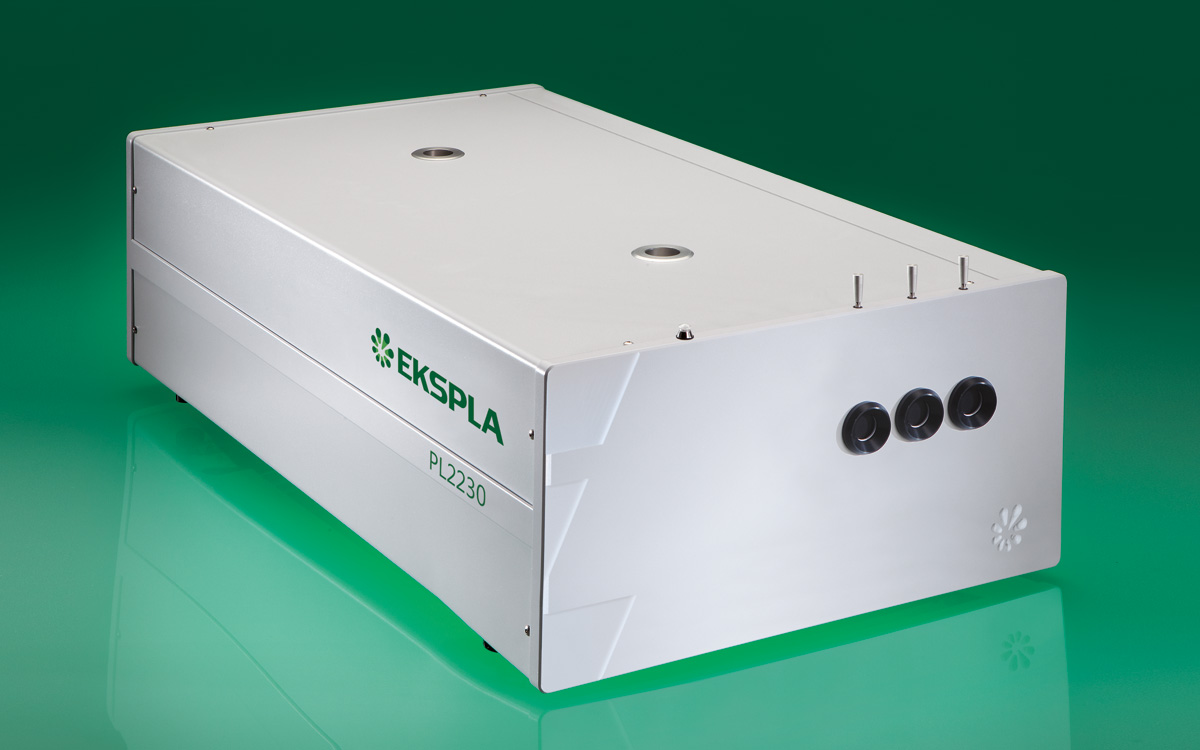
\includegraphics[width=\textwidth]{laser}
			\caption{Laser \emph{EKSPLA PL2231-50}.
% 				Převzato z~\autocite{ekspla-specs}.}
				Převzato z~\texttt{ekspla.com}.}
		\end{figure}
	\end{column}
	\end{columns}
\end{frame}

\section[E-FISH]{Electric field induced second harmonic generation}
\graphicspath{
	{../efish/}
	{img}
}

\begin{frame}
	\frametitle{E-FISH}
	\begin{columns}
	\begin{column}{0.5\textwidth}
		\begin{itemize}
			\item \emph{electric field-induced second harmonic generation}
			\item opticky nelineární prostředí nebo vysoká intenzita
			\item $\vec\epol = \epervac (\esusn1\vec\elfield + \esusn2\vec\elfield^2
% 				+ \esusn3\vec\elfield^3
				\ldots)$
			\item $\efish = \efishconst \ndens^2 \elfieldext^2 \itylaser^2$
		\end{itemize}
	\end{column}
	\begin{column}{0.5\textwidth}
		\includegraphics[width=\textwidth]{polarization}
	\end{column}
	\end{columns}
\end{frame}

\begin{frame}
	\frametitle{Zkoumaný výboj}
	\begin{columns}
	\begin{column}{0.6\textwidth}
		\includegraphics[width=\textwidth]{efish-reactor}
		\input{../efish/results/period-overview-full-small}
	\end{column}
	\begin{column}{0.4\textwidth}
		\begin{itemize}
			\item Townsendův výboj (DBD)
			\item sklo \SI{1.1}{\milli\metre} (2\times)
			\item mezera \SI{1}{\milli\metre}
			\item elektrody \num{14}\times\SI{15}{\milli\metre}
			\item \ce{N2}, \SI{3500}{\sccm}, \SI{1}{\atmosphere}
			\item \SI{11}{\kilo\hertz}, \SI{7}{\kilo\volt},
				\SI{3}{\milli\ampere}
			\item laser \SI{50}{\hertz}
		\end{itemize}
	\end{column}
	\end{columns}
\end{frame}

\begin{frame}
	\frametitle{Uspořádání experimentu}
	\includegraphics[width=\textwidth]{efish-setup}
\end{frame}

\begin{frame}
	\frametitle{Kalibrace}
	\input{../efish/results/period-calib-bilateral-small}
\end{frame}

\begin{frame}
	\frametitle{Výsledky}
	\begin{columns}
	\begin{column}{0.5\textwidth}
		\begin{figure}
			\centering
			\small
			signál \EFISH{} $\efish\,[\si{\arbunit}]$
			\medskip\par
			\input{../efish/results/period-efish-narrow}
		\end{figure}
	\end{column}
	\begin{column}{0.5\textwidth}
		\begin{figure}
			\centering
			\small
			elektrické pole $\elfield\,[\si{\mega\volt\per\metre}]$
			\medskip\par
			\input{../efish/results/period-elfield-narrow}
		\end{figure}
	\end{column}
	\end{columns}
\end{frame}

\begin{frame}
	\frametitle{Elektrické pole}
	\begin{figure}
		\centering
		\input{../efish/results/period-elfield-2d-small}
	\end{figure}
\end{frame}

\section{LIF}
\graphicspath{
	{../lif/}
	{img}
}

\begin{frame}
	\frametitle{Laserem indukovaná fluorescence}
	\small
	\begin{columns}
	\begin{column}{0.5\textwidth}
		\input{../lif/results/saturation-overall-small}
		\input{../lif/results/lifetime-example-small}
	\end{column}
	\begin{column}{0.5\textwidth}
		Určované parametry:
		\begin{itemize}
			\item saturační parametr $\lifsat$
			\item doba života $\lifetime$
			\item fluorescenční signál $\lif$
			\item prostorový profil svazku
			\item excitační profil
			\item spektrální překryv $\specoverlap$
		\end{itemize}
	\end{column}
	\end{columns}
\end{frame}

\section*{}

\begin{frame}
	\frametitle{Shrnutí}
	\begin{columns}[t]
	\begin{column}{0.5\textwidth}
		\EFISH
		\begin{itemize}
			\item úspěšná detekce signálu
			\item kalibrace ve známém poli
			\item parazitní signál z~okének
			\item aplikace na Townsendův výboj
			\item prostorově i~časově rozlišená intenzita elektrického pole
		\end{itemize}
	\end{column}
	\begin{column}{0.5\textwidth}
		LIF
		\begin{itemize}
			\item částečně saturovaný režim
			\item detekce selenových atomů ve vodíkovém plameni
			\item prostorové rozložení koncentrace \ce{Se}
			\item prostorová proměnlivost svazku
		\end{itemize}
	\end{column}
	\end{columns}
\end{frame}

\part{Otázky}
\section{Otázky}
\newcommand\question[1]{\begin{block}{Otázka}#1\end{block}}
\begin{frame}
	\partpage
\end{frame}

\begin{frame}
	\question{„Před kamerou se nacházela dvojice křemenných sklíček, která
		sloužila jako filtr pro odstínění rozptýleného laserového světla“:
		Jaká byla (zhruba) účinnost odstínění?}
	\begin{columns}
	\begin{column}{0.75\textwidth}
		\input{img/camerafilter}
	\end{column}
	\begin{column}{0.25\textwidth}
		\begin{align*}
			\transmittance{}_1 &= \num{0.242} \\
			\transmittance{}_2 &= \num{0.256} \\
			\transmittance{}_1 \transmittance{}_2 &= \num{0.062} \\
			\eta &= \SI{93.8}{\percent}
		\end{align*}
	\end{column}
	\end{columns}
\end{frame}

\begin{frame}
	\question{„[\ldots] byly všechny snímky korigovány odečtením temného
		snímku změřeného s vypnutým laserem“:
		Jak významná byla tato korekce a jaká byla opakovatelnost
		velikosti této korekce?}
\end{frame}

\begin{frame}
	\question{„Energie byla následně zprůměrována v časových intervalech
		odpovídajících jednotlivým snímkům kamery“:
		Znamená to, že energie jednotlivých pulzů nebyla stejná?
		Jaký byl (zhruba) rozptyl energie jednotlivých pulzů vyjádřený
		např.~jako relativní standardní odchylka?}
\end{frame}

\begin{frame}
	\question{„[\ldots] intenzita byla mnohem větší než u prostého plamene“:
		Máte pro to vysvětlení?}
	Chyba v~textu, umístění věty je zavádějící.
	Porovnává Rayleighův rozptyl a~vlastní záření plamene (bez laseru).
	\small
	\begin{columns}[t]
	\begin{column}{0.5\textwidth}
		\input{../lif/results/compare-flame-small}
		\smallskip\par
		Prostý plamen bez~laseru. Kamera bez~filtru, 10000 akumulací.
	\end{column}
	\begin{column}{0.5\textwidth}
		\input{../lif/results/compare-rayleigh-small}
		\smallskip\par
		Rayleighův rozptyl. Kamera bez~filtru, 100 akumulací.
	\end{column}
	\end{columns}
\end{frame}

\appendix
\begin{frame}
	\partpage
\end{frame}

\section{LIF}
\providecommand\vol{V}
\providecommand\sensabs{D_\text{a}}
\providecommand\lifsens{D_\text{F}}
\providecommand\rayleighsens{D_\text{R}}
\providecommand\lifsignal{M_\text{F}}
\providecommand\rayleighsignal{M_\text{R}}
\providecommand\rayleighndens{\ndens_\text{R}}
\providecommand\beamprofile{s}

\begin{frame}
	\frametitle{Prostorový profil svazku}
	\begin{columns}
	\begin{column}{0.5\textwidth}
		\centering
		naměřený profil
		\resizebox{\textwidth}{!}{
			\input{../lif/results/rayleigh-profile-s}
		}
	\end{column}
	\begin{column}{0.5\textwidth}
		\centering
		normovaný profil
		\resizebox{\textwidth}{!}{
			\input{../lif/results/rayleigh-profile-norm-s}
		}
	\end{column}
	\end{columns}
\end{frame}

\begin{frame}
	\frametitle{Příprava selenu}
	\begin{columns}[c]
	\begin{column}{1\textwidth}
		\begin{itemize}
			\item vzorek: roztok 10 ppb \ce{Se}
				v~\SI[per-mode=symbol]{1}{\mol\per\litre} \ce{HCl}
			\item reaguje s~borohydridem
				(\SI{0.5}{\percent} \ce{BH4} v~$0,4\%$ \ce{KOH})
				na~\ce{SeH2}
			\item nosný plyn: argon (\SI{775}{\sccm})
			\item přidán vodík (\SI{300}{\sccm})
			\item atomizace ve~vodíkovém plameni
				\begin{align*}
					\ce{
						H + SeH2 &-> H2 + SeH \\
						H + SeH &-> H2 + Se
					}
				\end{align*}
		\end{itemize}
	\end{column}
	\end{columns}
\end{frame}

\begin{frame}
	\frametitle{Chemická aparatura}
	\includegraphics[width=\textwidth]{img/lif-generator}
\end{frame}

\begin{frame}
	\frametitle{Excitační schéma}
	\centering
	\begin{tikzpicture}[scale=0.5]
		\small
		\seleniumlifgrotrian
	\end{tikzpicture}
\end{frame}

\begin{frame}
	\frametitle{Časový vývoj}
	\begin{columns}[c]
	\begin{column}{0.5\textwidth}
		\centering
		\includegraphics[height=0.28\textheight]{../lif/results/timeev-5.0.png}
		\includegraphics[height=0.28\textheight]{../lif/results/timeev-5.5.png}
		\includegraphics[height=0.28\textheight]{../lif/results/timeev-6.0.png}
	\end{column}
	\begin{column}{0.5\textwidth}
		\centering
		\includegraphics[height=0.28\textheight]{../lif/results/timeev-7.0.png}
		\includegraphics[height=0.28\textheight]{../lif/results/timeev-10.0.png}
		\includegraphics[height=0.28\textheight]{../lif/results/timeev-12.0.png}
	\end{column}
	\end{columns}
\end{frame}

\begin{frame}
	\frametitle{Určení koncentrace}
	Tříhladinový model v~lineárním režimu:
	\begin{align*}
		&\text{LIF:} &
		\lifsignal &= \einsteina32\,\lifetime
		\frac{\specoverlap \einsteinb13}{\lightspeed}
		\ndens \enlaser \lifeff
		\iiint_\vol \sensabs \frac{\solidangle}{4\pi} \beamprofile \dd{\vol} \\
		&\text{Rayleigh:} &
		\rayleighsignal &= \rayleighdxsect \, \rayleighndens
		\frac{\enlaserrayleigh}{\planck\freq} \, \rayleigheff
		\iiint_\vol \sensabs \solidangle \beamprofile \dd{\vol}
	\end{align*}
	\vspace{-3ex}
	\begin{block}{\vspace*{-2ex}}
		\begin{equation*}
			\ndens = \frac{\lifsignal}{\rayleighsignal}
			\frac{\enlaserrayleigh}{\enlaser}\frac{\rayleigheff}{\lifeff}
			\frac{1}{\einsteina32\,\tau}
			\frac{\lightspeed}{\planck\freq\specoverlap \einsteinb13}
			\, 4\pi \rayleighdxsect \frac{\pres}{\boltzmann\temp}
		\end{equation*}
	\end{block}
	\medskip
	\small
	\centering
	\begin{tabular}{l l l l}
		$\lifsignal$, $\rayleighsignal$ & měřený signál &
		$\specoverlap = \int l(\freq)\,a(\freq) \dd{\freq}$
			& spektrální překryv \\
		$\enlaser$, $\enlaserrayleigh$ & energie pulzu &
		$\beamprofile$\quad($\iint_S \beamprofile \dd S = 1$) & profil svazku \\
		$\lifeff$, $\rayleigheff$ & citlivost detektoru &
		$\solidangle$ & prostorový úhel \\
		$\sensabs$ & konstanta citlivosti &
		$\einsteina32$, $\einsteinb13$ & Einsteinovy koef. \\
	\end{tabular}
\end{frame}

\end{document}
